\documentclass{beamer}
\usepackage{biblatex}
\usepackage{tikz}
\usetikzlibrary{positioning}

\title[Virtual Lab Design and Lessons Learned]{%
  Thoughts on Virtual Lab Design during the Pandemic
}
\subtitle{Lessons Learned}
%\subtitle{Interactive Learning during COVID-19}
\author[R. S. D'Souza --- rollen.dsouza@uwaterloo.ca]{%
  Rollen S. D'Souza (\texttt{rollen.dsouza@uwaterloo.ca})
}
\date{June 17, 2021}
\addbibresource{references.bib} 
%%%%%%%%%%%%%%%%%%%%%%%%%%%%%%%%%%%%%%%%%%%%%%%%%%%%%%%%%%%%%%%%%%%%%%
%% BEGIN : ECE THEME
%%

% Slide style
\usetheme{Berlin}

% Color Scheme (UW Eng Colours)
\definecolor{UWEngPrimary}{cmyk}{.78,.94,0,0}
\definecolor{UWEngSecondary}{cmyk}{.60,.72,0,0}
\definecolor{UWEngTertiary}{cmyk}{0,0,0,1}

\setbeamercolor{palette primary}{bg=UWEngPrimary}
\setbeamercolor{palette secondary}{bg=UWEngSecondary}
\setbeamercolor{palette tertiary}{bg=UWEngTertiary}
\setbeamercolor{palette quaternary}{%
  fg=UWEngSecondary!5!white!95,%
  bg=UWEngPrimary!5!black!95%
}
\setbeamercolor{background canvas}{bg=UWEngTertiary!5!white!95}
\setbeamertemplate{itemize items}[circle]
\setbeamertemplate{enumerate items}[circle]
\setbeamercolor{itemize item}{fg=UWEngPrimary}
\setbeamercolor{itemize subitem}{fg=UWEngPrimary}
\setbeamercolor{itemize subsubitem}{fg=UWEngPrimary}
\setbeamercolor{item projected}{bg=UWEngPrimary}
\setbeamercolor{subitem projected}{bg=UWEngPrimary}
\setbeamercolor{subsubitem projected}{bg=UWEngPrimary}
%%
%% END   : ECE THEME
%%%%%%%%%%%%%%%%%%%%%%%%%%%%%%%%%%%%%%%%%%%%%%%%%%%%%%%%%%%%%%%%%%%%%%

\begin{document}

\frame{\titlepage}

\section{Background}
% \begin{frame}{Outline}
%   \begin{itemize}
%     \item{The Objective of Traditional Labs}
%     \item{Going Online: Translating the Objectives}
%     \item{What we learned from students and from the experience}
%   \end{itemize}
% \end{frame}

\begin{frame}{Traditional Engineering Lab Work}
  \begin{itemize}
    \item{
      Students perform pre-lab preparation.
    }
    \item{
      Lab instructor presents key information about the systems and the lab procedure.
      % \only<3->{
      %   \color{UWEngPrimary}
      %   Direct but traditional teaching presence.
      % }
    }
    \item{
      Students, in pairs, perform guided lab work on physical systems.
      % \only<2->{
      %   \color{UWEngPrimary}
      %   Collaborative and experiential learning.
      % }
    }
    \item{
      Pairs perform the procedure with the ability to ask questions and,
      % \only<4->{
      %   \color{UWEngPrimary}
      %   Opportunity for inquiry based learning.
      % }
    }
    \item{
      collect their data and write their reports outside the lab.
      % \only<5->{
      %   \color{UWEngPrimary}
      %   Traditional assessment, but often acts as more of a record.
      % }
    }
  \end{itemize}
\end{frame}

\begin{frame}{Traditional Engineering Lab Work}
  \emph{Generally accepted wisdoms...}
  \begin{itemize}
    \item{
      \textbf{
        Labs add value by engaging students with the real world aspects of engineering.
      }
    }
    \pause
    \item{
      \textbf{
        Labs motivate students; give a ``feel'' for the domain.
      }
    }
  \end{itemize}
\end{frame}

\begin{frame}{The Objectives of Labratory Work}
  Some key goals:~\cite{Feisel2005}
  \begin{itemize}
    \item{
      Instrumentation: learning practical techniques and tools,
      %\pause {\color{UWEngPrimary}covered by the physical nature of experiment.}
    } \pause
    \item{
      Experimentation: developing, understanding and implementing procedures,
      %\pause {\color{UWEngPrimary}manuals, documentation providing guidance on procedure.}
    } \pause
    \item{
      Modelling: managing with imperfect models,
      %\pause {\color{UWEngPrimary}covered by the physical nature of experiment.}
    } \pause
    \item{
      Communication: writing and speaking about the lab,
      %\pause {\color{UWEngPrimary}covered by writing reports.}
    } \pause
    \item{
      Teamwork and Collaboration: working effectively in teams.
      %\pause {\color{UWEngPrimary}students working in pairs.}
    }
  \end{itemize}
\end{frame}

\section{Going Online}

\frame<1-2>[label=goingonline]{
  \frametitle{Going Online: Meeting the Objectives}
  How do we meet these objectives?
  \begin{itemize}
    \item{
      \color<2->{UWEngPrimary!50!white!50}
      Experimentation and Communication
    } \pause
    \item{
      \color<3->{UWEngPrimary!50!white!50}
      Instrumentation and Modelling
    } \pause
    \item{
      Teamwork and Collaboration
    }
  \end{itemize}
}

\begin{frame}{Instrumentation and Modelling}
  \begin{tikzpicture}[x=1cm, y=1cm]
    \node[at={(0,0)}, anchor=south west]{
      \includegraphics{InstrumentModelling.pdf}
    };
    \node[at={(5, 3)}, anchor=south west]{
      \begin{minipage}{5cm}
      \begin{itemize}
        \item{
          \color<2->{UWEngPrimary!50!white!50}
          Cannot practice physical instrumentation.
        }
        \item{
          \color<2->{UWEngPrimary!50!white!50}
          What software instrumentation will students have to use in the future?
        }
      \end{itemize}
      \end{minipage}
    };
    \node<2->[at={(5, 0)}, anchor=south west]{
      \begin{minipage}{5cm}
      \begin{itemize}
        \item{
          Physical models aren't available.
        }
        \item{
          Virtual models (simulations) can be too perfect.~\cite{Chen2010}
        }
      \end{itemize}
      \end{minipage}
    };
    \node[at={(0,-1)}, anchor=south west]{
      \emph{%
        \tiny%
        Vector graphics created by rawpixel.com and brgfx --- \href{https://www.freepik.com/vectors/icons}{www.freepik.com}
      }
    };
  \end{tikzpicture}
\end{frame}

\begin{frame}{Model Interaction}
  \begin{center}
  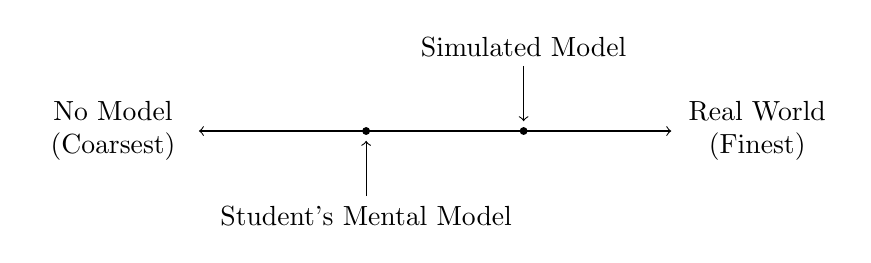
\begin{tikzpicture}
    \node[] (Coarse) {%
      \begin{minipage}{5.5em}
        \begin{center}No Model\\(Coarsest)\end{center}
      \end{minipage}%
    };
    \node[right={6cm of Coarse}] (Fine) {%
      \begin{minipage}{5.5em}
        \begin{center}Real World\\(Finest)\end{center}
      \end{minipage}%
    };
    \node[right={2cm of Coarse}] (StudentModel) {};
    \node[right={4cm of Coarse}] (InstructorModel) {};

    \draw[<->] (Coarse.east) -- (Fine.west);
    \fill (StudentModel.base) circle[radius=0.05cm];
    \fill (InstructorModel.base) circle[radius=0.05cm];

    \node[below={2em of StudentModel}] (StudentText) {
      Student's Mental Model
    };
    \draw[->] (StudentText.north) -- (StudentModel.south);
    \node[above={2em of InstructorModel}] (InstructorText) {
      Simulated Model
    };
    \draw[->] (InstructorText.south) -- (InstructorModel.north);
  \end{tikzpicture}
  \end{center}
  \pause
  % \begin{itemize}
  %   \item{Deterministic versus Probabilistic}%\pause
  %   \item{Linear versus Nonlinear}%\pause
  %   \item{Algebraic versus Differential}
  % \end{itemize}
  If chosen well (models are close enough) students can perform the lab while still experiencing ``real world'' effects.~\cite{Chen2010}
  Powerful; can consider scenarios not possible in a physical lab but exists in the real-world.
\end{frame}

\againframe<3>{goingonline}

\begin{frame}{Collaboration in Person}
  \begin{center}
    \includegraphics[page=1]{ThoughtExperiment.pdf}
  \end{center}
\end{frame}

\begin{frame}{Collaboration Online}
  \begin{center}
    \includegraphics[page=2]{ThoughtExperiment.pdf}
  \end{center}
\end{frame}

\section{Ending Thoughts}

\begin{frame}{Lessons as we go back in person...}
  \begin{itemize}
    \item{
      Are we incorporating modern instrumentation as well as we could?
    }
    \pause
    \item{
      Do we understand the precise difference between the student's mental model and the model presented in the lab (``real-world'')?
      Can we tune this to improve learning outcomes and blend virtual environments with physical environments?~\cite{Bumbacher2017,Olympiou2011}
    }
    \pause
    \item{
      Do we take as seriously the intergroup collaboration as we do intragroup collaboration? 
      Consider how to improve social presence~\cite{Fiock2020}.
    }
  \end{itemize}
\end{frame}

\renewcommand*{\bibfont}{\tiny}
\begin{frame}{References}{}
\printbibliography
\end{frame}
%Other thoughts. Labs are one of the aspects of higher education that are intrinsically tied to in-person instruction. If we do not have good labs, then the value of coming to Waterloo versus, taking a MOOC, becomes less clear (co-op aside). Not sure that is worth including, but I strongly believe that labs are a huge differentiator in terms of (engineering) education.

\end{document}